%!TEX root =  main.tex
\section{\dynastar}
%\section{Optimized dynamic state partitioning with \dynastar}
\label{sec:dynastar}

%In this section, we overview \dynastar's key ideas, present the protocol in detail, discuss some performance optimizations, and argue about \dynastar's correctness.
\subsection{Key insights}

\dynastar optimizes state partitioning based on the workload and relocates application state on-the-fly, without service disruption.
\begin{itemize}
\item \emph{Optimized state partitioning.}
\dynastar models a service workload as a graph $G = (V, E)$, where vertices represent state variables and edges dependencies between variables.
An edge connects two variables in the graph if a command accesses both of them.
A location oracle builds the workload graph based on feedback from the clients or partitions, as commands are executed.
The oracle periodically computes a partitioning of the workload graph and propagates the partitioning to the various partitions.

\item \emph{On-the-fly relocation of service state.}
Based on the partitioning computed by the oracle, servers determine the best partition to execute a multi-partition command.
State is then temporarily moved on demand to the destination partition where the command will be executed.
After the command is executed, updated variables are moved back to their source partition to keep the optimized partitioning.
When the oracle computes a new partitioning of the data, state is relocated (i.e., variables moved from one partition to another) to reflect the new optimized partitioning. 
\end{itemize}

%In \dynastar a move request is multicast together with the command that triggered the request.
%%a partition executes a command right after it has gathered all variables it needs.
%Therefore, differently from DS-SMR, \dynastar ensures termination without resorting to expensive mechanisms (i.e., S-SMR).

\subsection{Overview}
%\subsection{State partitioning as a graph problem}



\dynastar defines a dynamic mapping of variables to partitions (i.e., each variable is mapped to a partition).
Such a mapping is managed by a partitioning oracle, which is handled as a replicated partition.
%The oracle allows the mapping of variables to partitions to be retrieved or changed during execution.
To simplify the discussion, we initially assume that every command involves the oracle.
In \S\ref{sec:optm}, we explain how clients can use a cache to avoid the oracle in the execution of most commands.

\dynastar\ supports three types of commands:
$create(v)$ creates a new variable $v$ and initially maps it to a partition defined by the oracle;
$access(\omega)$ is an application command that reads and modifies variables in set $\omega \subseteq \vvm$; and
$delete(v)$ removes $v$ from the service state.
% resulting in $part(v) = \emptyset$,
% $move(v,\ppm_s,\ppm_d)$ moves variable $v$ from partition $\ppm_s$ to partition $\ppm_d$,
% and $consult(C)$ asks the oracle which variables are accessed by command $C$, and which partition contains each of them.

% The other possible values for a prophecy are $ok$ and $nok$, which mean that command can and cannot be executed, respectively (more details in Section~\ref{sec:algorithm}).
%If $v$ is not part of the service state (i.e., it was deleted or never created), the prophecy will contain~$\langle v, \emptyset \rangle$.

% explain which partitions deliver each partitioning command:
% how are access, consult, create, move and delete implemented?

%Once the oracle is in place, 
Clients submit commands to the oracle and wait for the reply. 
The reply from the oracle is called a $prophecy$, and usually 
consists of a set of tuples $\langle v, \ppm \rangle$, meaning 
$v \in \ppm$, and a target partition $\ppm_d$ on which the commands 
will be executed. The $prophecy$ could also tell the clients 
if a command cannot be executed (e.g., it accesses 
variables that do not exist). If the command can be executed, 
the clients wait for the reply from the target partition.

If a command $C$ accesses variables in $\omega$ on a single partition, 
the oracle forwards $C$ to that partition for execution. If the command 
accesses variables on multiple partitions, the oracle multicasts a 
$global(\omega,\ppm_d, C)$ command to the involved partitions to gather 
all variables in $\omega$ to one target partition. After having all 
required variables, the target partition executes command $C$, 
sends the reply to the client, and returns the variables to their source. 
Moving variables back to their source partitions improves the hit ratio of client caches (described in \S\ref{sec:optm}).

The oracle also collects hints from clients and partitions to 
build up the workload graph and monitors the changes in the graph. 
Periodically, the oracle computes a new optimized partitioning and sends the 
partitioning plan to all partitions. Upon delivering the new partitioning, 
the partitions exchange variables and update their state accordingly.
\dynastar relocates variables without blocking the execution of commands.

\subsection{The detailed protocol}
\label{sec:detailed}

Algorithms~\ref{alg:client_proxy}, \ref{alg:oracle_proxy}, and \ref{alg:server_proxy} describe the client, oracle, and server processes, respectively. 
For brevity, we omit the delete command since the coordination involved in the create and delete commands are analogous. 


\subsubsection{The client process} 

To execute a command, the client atomically multicasts the command to the oracle (Algorithm 1).
The oracle replies with a prophecy, which may already tell the client that the command cannot be executed (e.g., it needs a variable that does not exist, it tries to create a variable that already exists).
If the command can be executed, the client receives a prophecy containing the partition where the command will be executed. The client then waits for the result of the execution of the command.


% The client must retry the command if the partition cannot execute the command.
% This happens if the cache on client is invalid, some of the variables needed by the command were moved to another partition due a new partitioning. 
%To ensure that a command is eventually executed, after retrying a few times, the client falls back to using \ssmr{}, multicasting the command to all partitions (and the oracle, in case of a create or delete command).


\subsubsection{The oracle} 

When the oracle delivers a request, it distinguishes between two cases (Task 1 in Algorithm~\ref{alg:oracle_proxy}).
\begin{itemize}
\item If the command is to create a variable $v$, and $v$ does not already exist, the oracle chooses a random partition for $v$, multicasts the create command to the partition and itself, and returns the partition to the client as a prophecy (Figure~\ref{fig:oracle_repartition}).
\item If the command reads and writes existing variables, the oracle first checks that all such variables exist.
If the variables exist and they are all in a single partition, the oracle multicasts the command to that partition for execution.
If the variables are distributed in multiple partitions, the oracle deterministically determines the destination partition, and atomically multicasts a command to the involved partitions so that all variables are gathered at the destination partition.
Once the destination partition has received all variables needed by the command, it executes the command and returns the variables to their source partition.

%In either case, oracle returns a prophecy back to the client with the destination partition.
\end{itemize}


\begin{algorithm}[h!]
\small

\begin{distribalgo}[1]

%\vspace{1.0mm}

\INDENT{\colorbox{\coloralgo}{To issue a command $C$, the client does:}}

\vspace{1.0mm}
	% \STATE $\omega \leftarrow vars(C)$
	% \COMMENT{variables accessed by $C$}

	% \IF[if $v$ $\neg$exists in cache:]{$\exists v \in \omega : cache(\{v\}) = \bot$}
		\STATE \amcast$($oracle, $exec(C))$
		% \COMMENT{multicast command to $oracle$}
		\STATE wait for $prophecy$
		\IF[if receive $nok$ then...]{$prophecy = nok$}
			\STATE $reply \leftarrow prophecy$
			\COMMENT{...there's nothing to execute}
		\ELSE[in this case, $prophecy$ is $(dest)$]
			% \STATE $cache(\{v\}) \leftarrow prophecy$
			\STATE wait for $reponse$ from a server in $prophecy$
			\STATE $reply \leftarrow reponse$
		\ENDIF
	% \ELSE[if all vars in $\omega$ exist in cache]
	% 	\STATE $\ppm_d \leftarrow target(G_W, \omega)$
	% 	\COMMENT{select partition to execute}
	% 	\STATE \amcast$(\ppm_d, exec(C))$
	% 	\STATE wait for $reponse$ from server $\ppm_d$
	% 	\IF[if receive $retry$ then...]{$reponse = retry$}
	% 		\STATE $cache(\{v\}) \leftarrow \bot$
	% 		\COMMENT {clear cache of $\omega$}
	% 		\STATE return retry $C$
	% 	\ELSE
	% 		\STATE $reply \leftarrow reponse$
	% 	\ENDIF	

	% \ENDIF
\STATE return $reply$ to the application

\vspace{1.0mm}

% \INDENT{\colorbox{\coloralgo}{\textbf{function} cache$(vars)$}}
% 	\STATE $dests \leftarrow \{ \ppm : \exists v \in vars \cap \ppm \}$
% 	\STATE return $dests$
% \ENDINDENT

% \vspace{1.0mm}
% \INDENT{\colorbox{\coloralgo}{\textbf{function} target$(vars)$}}
% 	\STATE $\ppm \leftarrow$ compute destination partition for $vars$ from\\ \hspace{8mm}current $\ppm_1, ..., \ppm_m$ and $\ip_1, ..., \ip_m$ partitioning
% 	\STATE return $\ppm$
% \ENDINDENT	

\ENDINDENT

\caption{Client}
\label{alg:client_proxy}
\end{distribalgo}
\end{algorithm}
\begin{algorithm}[t!]
\small

\begin{distribalgo}[1]

%\vspace{1.0mm}

\INDENT[\textbf{Task 1}]{\colorbox{\coloralgo}{\textbf{when} \amdel$(exec(C))$}}
	\INDENT{\textbf{case} $C$ is a $create(v)$ command:}
		\IF[if $v$ already exists...]{$\parts(\{v\}) \neq \bot$}
			\STATE $prophecy \leftarrow nok$
			\COMMENT{...notify client}
		\ELSE[if $v$ doesn't exist...]
			\STATE $\ppm \leftarrow$ choose $v$'s partition
			\COMMENT{...determine $v$'s partition}
			\STATE $prophecy \leftarrow \ppm$
			\COMMENT{prepare client's response}
			\STATE $alldest \leftarrow \{oracle\} \cup \{ \ppm \}$
			\STATE \amcast$(alldest, (\ppm,create(v)))$
%					\COMMENT{send command to partition}
		\ENDIF
	\ENDINDENT

	\INDENT{\textbf{case} $C$ is any command, but $create(v)$:}
		\STATE $\omega \leftarrow vars(C)$
		\COMMENT{variables accessed by $C$}
		\IF[if $v$ $\neg$exists:]{$\exists v \in \omega : \parts(\{v\}) = \bot$}
			\STATE $prophecy \leftarrow nok$
			\COMMENT{tell the client}
		\ELSE[if all vars in $\omega$ exist]
			\STATE $dests \leftarrow \parts(\omega)$
			\COMMENT{get all partition involved}
			\STATE $\ppm_d \leftarrow target(dests, C)$
			\COMMENT{$\ppm_d$ will excecute $C$}
			\STATE \amcast$(dests, C)$
			\STATE $prophecy \leftarrow \ppm_d$
		\ENDIF
	\ENDINDENT
	\STATE send $prophecy$ to the client
\ENDINDENT
\vspace{1.0mm}

\INDENT[\textbf{Task 2}]{\colorbox{\coloralgo}{\textbf{when} \amdel$(\ppm_v,create(v))$}}
%	\INDENT{\textbf{case} $C$ is a $create(v)$ command:}
%	\STATE \rmcast$(\ppm_v, \langle signal, C \rangle )$
	\STATE $\forall x \in \ppm_v$: send $(\langle signal, C \rangle )$ to $x$
	\COMMENT{exchange signal...}
	\STATE wait until $\langle signal, C \rangle \in rcvd\_msgs$
	\COMMENT{...to coordinate}
	\STATE $\ppm_v \leftarrow \ppm_v \cup      \{v\}$
% \STATE send $ok$ to the client
\ENDINDENT


\vspace{1.0mm}
\INDENT[\textbf{Task 3}]{\colorbox{\coloralgo}{\textbf{when} receive $( \langle val, C \rangle )$}}
%\INDENT[\textbf{Task 3}]{\colorbox{\coloralgo}{\textbf{when} \rmdel$( \langle val, C \rangle )$}}
	\STATE $rcvd\_msgs \leftarrow rcvd\_msgs \cup \{\langle val, C \rangle\}$
\ENDINDENT

\vspace{1.0mm}
\INDENT{\colorbox{\coloralgo}{\textbf{function} \parts$(vars)$}}
	\STATE $dests \leftarrow \{ \ppm : \exists v \in vars \cap \ppm \}$
	\STATE return $dests$
\ENDINDENT

	\vspace{1.0mm}

\INDENT[\textbf{Task 4}]{\colorbox{\coloralgo}{\textbf{when} \amdel$(hint(V_h,E_h))$}}
	\STATE update $G_W$ with $(V_h,E_h)$
	\STATE $inc(changes)$
	\IF {$changes \geq threshold$}
		\STATE $partitioning  \leftarrow$ compute $\ip_1, ..., \ip_m$ from $G_W$
		\STATE $alldest \leftarrow \{oracle\} \cup all partitions$
		\STATE \amcast$(alldest, (partitioning))$
	\ENDIF
\ENDINDENT

\vspace{1.0mm}

\INDENT[\textbf{Task 5}]{\colorbox{\coloralgo}{\textbf{when} \amdel$(\mathit{partitioning})$}}
	\STATE apply $partitioning$
\ENDINDENT

\vspace{1.0mm}

\INDENT{\colorbox{\coloralgo}{\textbf{function} target$(\ppm, C)$}}
	\STATE $\ppm_d \leftarrow$ deterministicly compute partition to execute\\ \hspace{8mm} command $C$ from $\forall \ppm_i \in \ppm$
	\STATE return $\ppm_d$
\ENDINDENT	

\vspace{1.5mm}

\textbf{Algorithm variables:}

\vspace{1mm}

$G_W$: the set of all variable and their locations

$partitioning$: the partition configuration of $G_W$


\caption{Oracle}
\label{alg:oracle_proxy}
\end{distribalgo}
\end{algorithm}




\begin{algorithm}[t!]
\small

\begin{distribalgo}[1]

\INDENT[\textbf{Task 1}]{\colorbox{\coloralgo}{\textbf{when} \amdel$(access(\omega))$}}
	% \IF{$\forall v \in \omega : v \in \ppm$}
		\STATE execute command $access(\omega)$
		\STATE send response to the client
	% \ELSE
		% \STATE send $retry$ to the client
	% \ENDIF
\ENDINDENT
\vspace{1.0mm}
	\INDENT[\textbf{Task 2}]{\colorbox{\coloralgo}{\textbf{when} \amdel$(move(\omega,dests,\ppm_d), access(\omega))$}}
%	\INDENT{\textbf{case} $C$ is a $move(v,\ppm_s,\ppm_d)$ command:}
		\IF[if $\ppm$ is a source partition:]{$\ppm \in dests \setminus \ppm_d$}
			\STATE $vars \leftarrow \omega \cap \ppm$
			\COMMENT{all needed variables in $\ppm$}
			\STATE \rmcast$(\ppm_d$,$\langle vars, C \rangle)$
			\COMMENT{send variables to destination}
			\STATE $\ppm \leftarrow \ppm \setminus \omega$
			\COMMENT{update source partition}
		\ELSE[$\ppm$ is destination partition:]
			\STATE wait until $\exists vars : \langle vars, C \rangle \in rcvd\_msgs$
				\STATE $\ppm \leftarrow \ppm \cup vars$
				\COMMENT{update partition}
				\STATE execute command $access(\omega)$
				\STATE send response to the client
		\ENDIF
	\ENDINDENT
	\vspace{1.0mm}
	\INDENT[\textbf{Task 3}]{\colorbox{\coloralgo}{\textbf{when} \amdel$(create(v))$}}
		\STATE $\ppm \leftarrow \ppm \cup \{v\}$
		\STATE send $ok$ to the client
	\ENDINDENT
%	\vspace{1.0mm}
%	\INDENT{\textbf{case} $C$ is a $delete(v)$ command:}
%		\STATE wait until $\langle val, C \rangle \in rcvd\_msgs$
%                \STATE $\ppm \leftarrow \ppm \setminus \{v\}$
%                \STATE send $ok$ to the client
%		\STATE \rmcast$(oracle, \langle ok, C \rangle )$
%        	\ENDINDENT
%\ENDINDENT

  \vspace{1.0mm}

  \INDENT[\textbf{Task 4}]{\colorbox{\coloralgo}{\textbf{when} \rmdel$( \langle val, C \rangle )$}}
      \STATE $rcvd\_msgs \leftarrow rcvd\_msgs \cup \{\langle val, C \rangle\}$
  \ENDINDENT

%\ENDINDENT

\caption{Server in partition $\ppm$}
\label{alg:server_proxy}
\end{distribalgo}
\end{algorithm}

\begin{figure*}
\begin{minipage}[b]{1\linewidth} % A minipage that covers the whole width of the page
\centering
      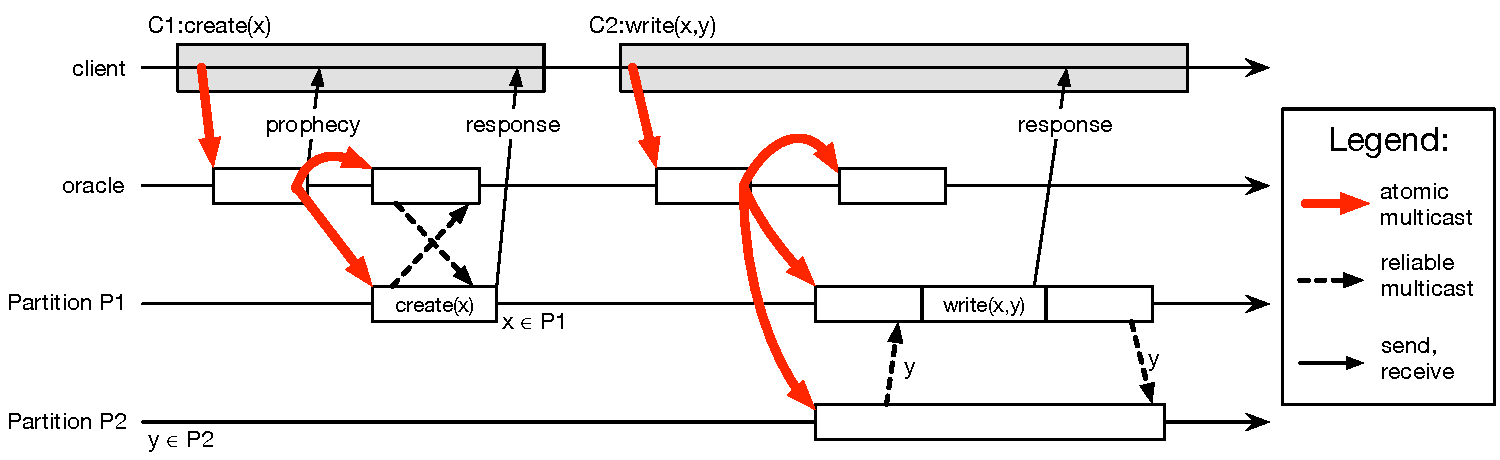
\includegraphics[width=\linewidth]{figures/dynastar}
\end{minipage}
\caption{The execution of a create (C1) and a write without client cache (C2) and with client cache (C3) in \dynastar.}
\label{fig:oracle_repartition}
\end{figure*}

Upon delivering a create (Task 2), the oracle updates its partition information.
As part of a create command, the oracle coordinates with the partition to ensure correctness (Task 3)~\cite{bezerra2014ssmr}.
%
The oracle also keeps track of the workload graph by receiving hints with variables (i.e., vertices in the graph) and executing commands (i.e., edges in the graph). These hints can be submitted by the clients or by the partitions, which collect data upon executing commands and periodically inform the oracle (Task 4).
The oracle computes a partitioning plan of the graph and multicasts it to all servers and to itself. Upon delivering new partition plan, the oracle updates its location map accordingly (Task 5).
% The oracle also keeps track of the workload graph, computes a partitioning of the graph, and determines the destination partition for move operations.
% To maintain the workload graph (Task 5), the oracle receives hints with variables (i.e., vertices in the graph) and executed commands (i.e., edges in the graph).

To compute an optimized partitioning, the oracle uses a graph partitioner.
A new partitioning can be requested by the application, by a partition, or by the oracle itself (e.g., upon delivering a certain number of hints).
To determine the destination partition of a set of variables, as part of a move, the oracle uses 
% the current location of variables and 
the last computed partitioning.

\subsubsection{The server process} 

When a server delivers a command $C$, it first checks if it has all variables needed by the command. If the server has all such variables, it executes the command and sends the response back to the client (Tasks 1a and 2 in Algorithm~\ref{alg:server_proxy}).
If not all the variables needed by the command are in that partition, the server runs a deterministic function to determine the destination partition to execute the command (Task 1b). The function uses as input the variables needed by the command and the command itself.
In this case, each server that is in the multicast group of the command $C$ but is not the destination partition sends all the needed variables stored locally to the destination partition and waits to receive them back. 
The destination partition waits for a message from other partitions. Once all variables needed are available, the destination partition executes the command $C$, sends the response back to the client, and returns the variables to their source.
Periodically, the servers deliver a new partitioning plan from the oracle (Task 3). Each server will send the variables to the designated partition, as in the plan, and wait for variables from other partitions. Once a server receives all variables, it updates its location map accordingly.
%When a server delivers a message to create a variable (and similarly to delete an existing variable), it coordinates with the oracle (Task 3).
%The exchange of signals between the partition where the variable will be created and the oracle ensures that interleaved executions between create and delete commands will not lead to violations of linearizability (i.e., this is essentially the execution of a multi-partition command involving the oracle and a partition~\cite{bezerra2014ssmr}).
To determine the destination partition for a command, the servers uses the last computed partitioning.


\subsection{Performance optimization}
%\subsection{Performance optimizations}
\label{sec:optm}

%We now describe two performance optimizations.
%
%\textbf{Caching.} 
In the algorithm presented in the previous section, clients always need to involve the oracle, and the oracle dispatches every command to the partitions for execution.
Obviously, if every command involves the oracle, the system is unlikely to scale, as the oracle will likely become a bottleneck.
To address this issue, clients are equipped with a location cache.
Before submitting a command to the oracle, the client checks its location cache.
If the cache contains the partition of the variables needed by the command, the client can atomically multicast the command to the involved partition and thereby avoid contacting the oracle. 

The client still needs to contact the oracle in one of these situations:
%(a)~according to client's cache, not all variables accessed by the command are in the same partition and it is necessary to move variables;
%(b)~the cache contains outdated information, and the command is multicast to a partition that does not contain all needed variables; or
(a)~the cache contains outdated information; or
(b)~the command is a create, in which case it must involve the oracle, as explained before.
%If the cache contains outdated information and the addressed partition does not contain all the variables accessed by the command, the partition tells the client to retry the command.
If the cache contains outdated information, it may address a partition that does not have the information of all the variables accessed by the command.
In this case, the addressed partition tells the client to retry the command.
The client then contacts the oracle and updates its cache with the oracle's response.
Although outdated cache information results in execution overhead, it is expected to happen rarely since repartitioning is not frequent.

%\textbf{Subgraph on servers}. If all partitions have to keep a copy of the the workload graph, scaling is also a problem if the graph grows over time. Thus, servers only keep a subgraph of variables they hold and the neighbors of those objects, by observing the access pattern of the commands. Using this subgraph only, the servers can compute the destination partition for commands without the need of the full graph.





